%%%%%%%%%%%%%%%%%%%%%%%%%%%%%%%%%%%%%%%%%%%%%%%%%%%%%%%%%%%%%%%%%%%%%
%                                                                   %
%	CHAPTER ONE, MODELS of HPC                                       %
%                                                                   %
%%%%%%%%%%%%%%%%%%%%%%%%%%%%%%%%%%%%%%%%%%%%%%%%%%%%%%%%%%%%%%%%%%%%%

\chapter{Models for HPC}

\section{Introduction}

High Performance Computing (HPC) takes its roots from the beginning of computer odyssey in the middle of 20th century.
From this emerged rules, observations, theories, and most computer science fields.
Knowledge of the theory is required to understand and characterize HPC and supercomputers.  
This part describes the Von Neumann model, the generic model of sequential computer on which every modern machine is built.
The Von Neumann model, along with the Flynn taxonomy which is the classification of the different execution models, will be presented. 
We also review the different memory models based on those elements. 

Parallelism will be discussed in detail and we present how it can be used to reach performances, and thus examine what performance implies in HPC.
The Amdahl's and Gustafson's laws are presented in detail, along with the strong and weak scaling used in our study. 

\section{Von Neumann Model}
\index{Von Neumann Model}
The first early 20\textsuperscript{th} century computers were built using vacuum tubes making them high power consuming, and therefore were hard to maintain and expensive to build.
The most famous of first vacuum tubes supercomputers, the ENIAC, was based on a decimal system.
As well-known as this supercomputer may be, the real revolution came from its successor.
The first binary system based computer was created in 1944 and was called the Electric Discrete Variable Automatic Computer (EDVAC). 
A physicist from the EDVAC team a described the logical model of this computer and provided a model on which every modern computing device is based. 

\begin{figure}
\centering 
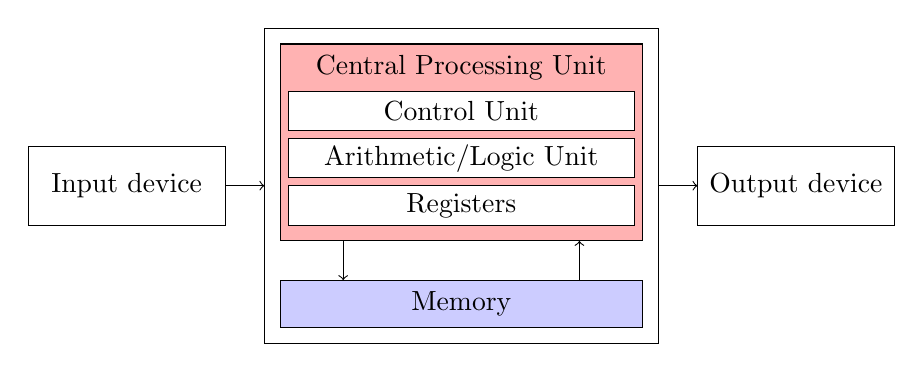
\begin{tikzpicture}
\draw (3,0) rectangle (8,4);
\draw (3.2,1.3) [fill=red!30] rectangle (7.8,3.8);
\node at (5.5,3.5) {Central Processing Unit};

\draw (3.3,1.5) [fill=white] rectangle (7.7,2.) node[pos=.5] {Registers};
\draw (3.3,2.1) [fill=white] rectangle (7.7,2.6) node[pos=.5] {Arithmetic/Logic Unit};
\draw (3.3,2.7) [fill=white] rectangle (7.7,3.2) node[pos=.5] {Control Unit};

\draw (0,1.5) rectangle (2.5,2.5) node[pos=.5] {Input device};
\draw (8.5,1.5) rectangle (11,2.5) node[pos=.5] {Output device};
\draw [->] (2.5,2) -- (3,2);
\draw [->] (8,2) -- (8.5,2);

\draw (3.2,.2) [fill=blue!20] rectangle (7.8,.8) node[pos=.5] {Memory};
\draw [->] (4,1.3) -- (4,.8);
\draw [->] (7,.8) -- (7,1.3);
\end{tikzpicture}
\caption{Von Neumann model}
\label{fig:1_HPC:von_neumann_model}
\end{figure}

John Von Neumann published the \textit{First Draft of a Report on the EDVAC}~\cite{von1993first} in 1945. 
The model known as the Von Neumann model, more commonly referred as the Von Neumann Machine, came from this work.
The model is presented on figure~\ref{fig:1_HPC:von_neumann_model}.

The figure has tree identified parts: the input and output devices and, in the middle, the computational device itself in the middle. 
\paragraph{Input/Output devices}
The input and output devices are used to store data in a read/write way. 
They can be represented as hard drives, solid state drives, monitors, printers or even mouse and keyboard.
The input and output devices can also be the same, reading and writing in the same area.\\

\paragraph{Memory} 
Inside the computational unit we find the general memory to store program and data. 
The most common architectures it can be considered as a Random Access Memory (RAM). 
There are several types of memory and will be discussed later in this thesis. 

\paragraph{Central Processing Unit}
\index{Central Processing Unit}
The Central Processing Unit (CPU) is composed of several elements in this model. 
\begin{itemize}[noitemsep,nolistsep]
\item[-] On one hand, the \textit{Arithmetic and Logic Unit} (ALU) takes as input one or two values, the data and applies an operation on them. 
The operation can be either logic with operators such as AND, OR, XOR, etc. or arithmetic with operators such as ADD, MUL, SUB, etc. 
These operators may be more complex on modern CPUs. 
\item[-] Conversely, we find the \textit{Control Unit} (CU) which controls the data carriage to the ALU from the memory and the operation to be performed on data.
It is also involved in the Program Counter (PC), which is the address of the next instruction in the program. 
\item[-] We can identify the \textit{Registers} section which represents data location used for both ALU and CU to store temporary results, the current instruction address, etc. 
Some representations may vary since the \textit{Registers} can be represented directly inside the ALU or the CU. 
\end{itemize}
\paragraph{Buses}
The links between those elements are called buses and can be separated in data buses, control buses and addresses buses.
These will have a huge importance for the first machines optimizations, growing the size of the buses from 2, 8, 16, 32, 64 and even more for vector machines with 128 and 256 bits.\\

The usual processing flow on such architectures can be summarized as a loop: 
\begin{itemize}[noitemsep,nolistsep]
\item[-] Fetch instruction at current PC from memory;
\item[-] Decode instruction using the Instruction Set Architecture (ISA). The main ISA are Reduce Instruction Set Computer architecture (RISC) and Complex Instruction Set Computer architecture (CISC);
\item[-] Evaluate operand(s) address(es);
\item[-] Fetch operand(s) from memory;
\item[-] Execute operation(s).
\item[-] Store results, increase PC.\\
\end{itemize}

With the instruction sets and new architectures, several similar operations can be processed in the same clock time.
Every device or machine we describe in the next chapter has this architecture as a basis. 
One will consider execution models and architecture models to characterize HPC architectures.

\section{Flynn taxonomy and execution models}
\index{Flynn taxonomy}
The Von Neumann model gives us a general idea of how a computational unit is fashioned. 
The constant demand for more powerful computers required scientists to find different ways to provide this computational power.
In 2001, IBM proposed the first multi-core processor on the same die: the Power4 with its 2 cores.
This evolution required new paradigms.
A right characterization become essential to be able to target the right architecture for the right purpose. 
The Flynn taxonomy presents a hierarchical organization of computation machines and executions models.

\begin{table}
\centering
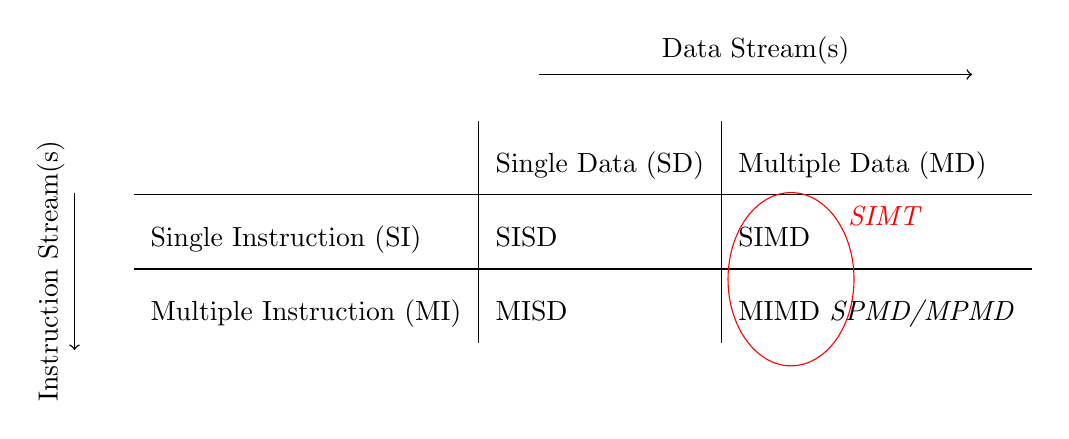
\begin{tikzpicture}
\node (table) {\arraycolsep=1.4pt\def\arraystretch{2.2}
\begin{tabular}{l | l | l}
 & Single Data (SD) & Multiple Data (MD) \\
 \hline 
Single Instruction (SI) & SISD & SIMD \\
\hline 
Multiple Instruction (MI) & MISD & MIMD \textit{SPMD/MPMD} \\
\end{tabular}
};
\draw [->,line width=.5pt] (-0.5,2) -- (5,2) node[midway, above] {Data Stream(s)};
\draw [->,line width=.5pt] (-6.4,0.5) -- (-6.4,-1.5) node[rotate=180,sloped, midway, above] {Instruction Stream(s)};
\draw [red] (2.7,-.6) ellipse (.8cm and 1.1cm) node[xshift=1.2cm,yshift=.8cm] {\textit{SIMT}};
%\draw[decoration={brace,raise=5pt},line width=1pt,decorate]
%  (5,0.4) -- node[right=6pt,yshift=5pt] {\textit{SIMT}} (5,-1.5);
\end{tikzpicture}
\caption{Flynn taxonomy for execution models completed with SPMD and SIMT models}
\label{tab:1_HPC:taxonomy_flynn}
\end{table}

\begin{figure}
\resizebox {.24\columnwidth} {!} {
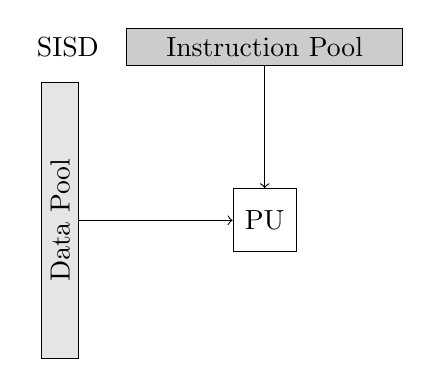
\begin{tikzpicture}
\draw (0.1,5.2) node {SISD}; 
\node (rect) at (2.6,5.2) [draw,minimum width=3.5cm,fill=black!20] (ip) {Instruction Pool};
\node (rect) at (0,3) [rotate=90,draw,minimum width=3.5cm,fill=black!10] (dp) {Data Pool};
\node (rect) at (2.6,3) [draw,minimum width=.8cm,minimum height=.8cm] (pu1) {PU};
\draw [->] (ip) -- (pu1);
\draw [->] (dp) -- (pu1);
\end{tikzpicture}
}
\resizebox {.24\columnwidth} {!} {
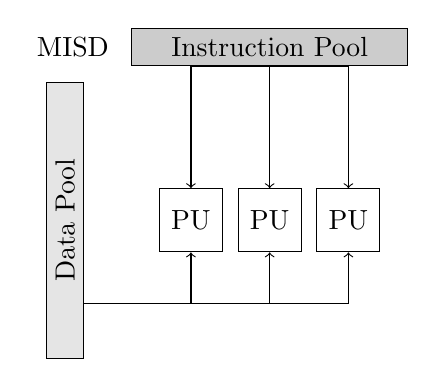
\begin{tikzpicture}
\draw (0.1,5.2) node {MISD}; 
\node (rect) at (2.6,5.2) [draw,minimum width=3.5cm,fill=black!20] (ip) {Instruction Pool};
\node (rect) at (0,3) [rotate=90,draw,minimum width=3.5cm,fill=black!10] (dp) {Data Pool};
\node (rect) at (1.6,3) [draw,minimum width=.8cm,minimum height=.8cm] (pu1) {PU};
\node (rect) at (3.6,3) [draw,minimum width=.8cm,minimum height=.8cm] (pu2) {PU};
\node (rect) at (2.6,3) [draw,minimum width=.8cm,minimum height=.8cm] (pu3) {PU};

\draw[<-] (pu1.north) |-  (ip.south); 
\draw[<-] (pu2.north) |-  (ip.south);
\draw[<-] (pu3.north) |-  (ip.south);

\draw[<-]  (pu1.south) |- ([yshift=-30pt]dp.south);
\draw[<-]  (pu2.south) |- ([yshift=-30pt]dp.south);
\draw[<-]  (pu3.south) |- ([yshift=-30pt]dp.south);

\end{tikzpicture}
}
\resizebox {.24\columnwidth} {!} {
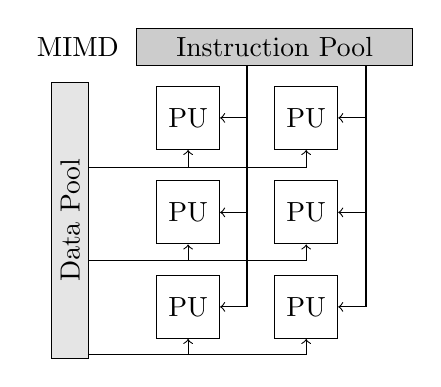
\begin{tikzpicture}
\draw (0.1,5.2) node {MIMD}; 
\node (rect) at (2.6,5.2) [draw,minimum width=3.5cm,fill=black!20] (ip) {Instruction Pool};
\node (rect) at (0,3) [rotate=90,draw,minimum width=3.5cm,fill=black!10] (dp) {Data Pool};
\node (rect) at (1.5,4.3) [draw,minimum width=.8cm,minimum height=.8cm] (pu1) {PU};
\node (rect) at (1.5,3.1) [draw,minimum width=.8cm,minimum height=.8cm] (pu2) {PU};
\node (rect) at (1.5,1.9) [draw,minimum width=.8cm,minimum height=.8cm] (pu3) {PU};
\node (rect) at (3,4.3) [draw,minimum width=.8cm,minimum height=.8cm] (pu4) {PU};
\node (rect) at (3,3.1) [draw,minimum width=.8cm,minimum height=.8cm] (pu5) {PU};
\node (rect) at (3,1.9) [draw,minimum width=.8cm,minimum height=.8cm] (pu6) {PU};

\draw[<-]  (pu1.south) |- ([yshift=19pt]dp.south);
\draw[<-]  (pu4.south) |- ([yshift=19pt]dp.south);

\draw[<-]  (pu2.south) |- ([yshift=-14.5pt]dp.south);
\draw[<-]  (pu5.south) |- ([yshift=-14.5pt]dp.south);

\draw[<-]  (pu3.south) |- ([yshift=-48.5pt]dp.south);
\draw[<-]  (pu6.south) |- ([yshift=-48.5pt]dp.south);

\draw[->] ([xshift=-10pt]ip.south) |- (pu1.east);
\draw[->] ([xshift=-10pt]ip.south) |- (pu2.east);
\draw[->] ([xshift=-10pt]ip.south) |- (pu3.east);

\draw[->] ([xshift=33pt]ip.south) |- (pu4.east);
\draw[->] ([xshift=33pt]ip.south) |- (pu5.east);
\draw[->] ([xshift=33pt]ip.south) |- (pu6.east);

%\draw[<-]  (pu2.south) |- ([yshift=-30pt]dp.south);
%\draw[<-]  (pu3.south) |- ([yshift=-30pt]dp.south);

%\draw [->] (ip) -- (pu1);
%\draw [->] (dp) -- (pu1);
\end{tikzpicture}
}
\resizebox {.24\columnwidth} {!} {
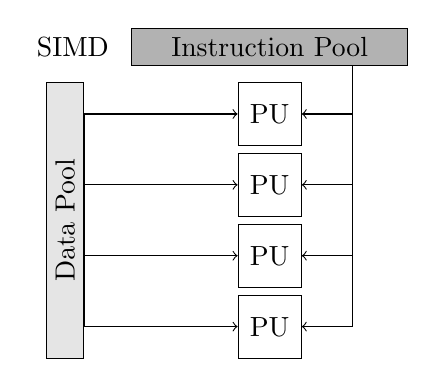
\begin{tikzpicture}
\draw (0.1,5.2) node {SIMD}; 
\node (rect) at (2.6,5.2) [draw,minimum width=3.5cm,fill=black!30] (ip) {Instruction Pool};
\node (rect) at (0,3) [rotate=90,draw,minimum width=3.5cm,fill=black!10] (dp) {Data Pool};
\node (rect) at (2.6,4.35) [draw,minimum width=.8cm,minimum height=.8cm] (pu1) {PU};
\node (rect) at (2.6,3.45) [draw,minimum width=.8cm,minimum height=.8cm] (pu2) {PU};
\node (rect) at (2.6,2.55) [draw,minimum width=.8cm,minimum height=.8cm] (pu3) {PU};
\node (rect) at (2.6,1.65) [draw,minimum width=.8cm,minimum height=.8cm] (pu4) {PU};
%\draw [->] ([yshift=2.35cm]dp) -- (pu1);
\draw[->] (dp.south) |- (pu1.west);
\draw[->] (dp.south) |- (pu2.west);
\draw[->] (dp.south) |- (pu3.west);
\draw[->] (dp.south) |- (pu4.west);

\draw[->] ([xshift=30pt]ip.south) |- (pu4.east);
\draw[->] ([xshift=30pt]ip.south) |- (pu3.east);
\draw[->] ([xshift=30pt]ip.south) |- (pu2.east);
\draw[->] ([xshift=30pt]ip.south) |- (pu1.east);
%\draw[arrow] (Small2B.north)--(Small2B|-Big2.south);s
%\draw [->] (dp) -- (pu1);
\end{tikzpicture}
}
\caption{Flynn taxonomy schematic representation of execution models}
\label{fig:1_HPC:flynn_taxonomy}
\end{figure}

In this classification~\cite{flynn1972some} from 1972, Michael J. Flynn presents the SISD, MISD, MIMD, and SIMD models.
Each of those execution models, presented on table~\ref{tab:1_HPC:taxonomy_flynn} and figure~\ref{fig:1_HPC:flynn_taxonomy}, corresponds to a specific machine and function.

\subsection{Single Instruction, Single Data: SISD}
The model corresponding to a single core CPU is similar to the Von Neumann model. 
This sequential model takes one instruction, operates on one data and the result is then stored before the process continues over. 
SISD is important to consider for a reference computational time and will be taken into account in the next part for Amdahl's and Gustafson's laws.

\subsection{Multiple Instructions, Single Data: MISD}
This model can correspond to a pipelined computer.
Different operation flows are applied to the datum, which is transferred to the next computational unit and so on. 
This is the least common execution model.


\subsection{Multiple Instructions, Multiple Data: MIMD}
Every element in MIMD executes its own instructions flow on its own data set. 
This can represent the behavior of a processor using several cores, threads or even the different nodes of a supercomputer cluster. 
Two subcategories are identified in this model: SPMD and MPMD.

\subsubsection{SPMD}
The Single Program Multiple Data model (SPMD), where each process executes the same program, is the most famous parallelism way for HPC purpose.
All programs are the same, but does not share the same instruction counter. 
SPMD was proposed for the first time in \cite{darema1988single} in 1988 using Fortran.
This is the common approach working with runtime like MPI. 
The programs are the same and the executions are independent but based on their ID the processes will target different data. 

\subsubsection{MPMD}
The Multiple Program Multiple Data (MPMD) model is also known for HPC.
MPMD involves some of the processes to execute different programs, generally with a separation between a main program generating data for sub-programs. 
This is the model on which we work in Part II, regarding the Langford problem resolution using a master program generating tasks for the slaves CPUs/GPGPUs programs.

\subsection{Single Instruction, Multiple Data: SIMD}
This execution model corresponds to many-core architectures like a GPU. 
SIMD can be extended from two to sixteen elements for classical CPUs to hundreds and even thousands of core for GPGPUs. 
In the same clock cycle, the same operation is executed on every process on different data. 
A good example is the work on matrices with stencils: the same instruction is executed on every element of the matrix in a synchronous way and the processing elements share one instruction unit and program counter. 

\subsection{SIMT}
\index{Single Instruction Multiple Threads}
Another characterization was determined to describe the new GPUs architecture: Single Instruction Multiple Threads. 
This first appears in one of NVIDIA's company paper~\cite{lindholm2008nvidia}. 
This model describes a combination of MIMD and SIMD architectures where every block of threads is working with the same control processor on different data and in such a way that every block has its own instruction counter.  
The model we describe in Part~\ref{sec:CUDA}, used for the \textit{warps} model in NVIDIA CUDA.

\section{Memory}
\label{sec:NORMA}
In addition to the execution model and parallelism, the memory access patterns have an important role in performances of SIMD and MIMD. 
In this classification we identify three categories: UMA, NUMA and NoRMA for shared and distributed cases. 
This classification has been pointed out in the Johnson's taxonomy\cite{johnson1988completing}.

\begin{figure}
\centering 
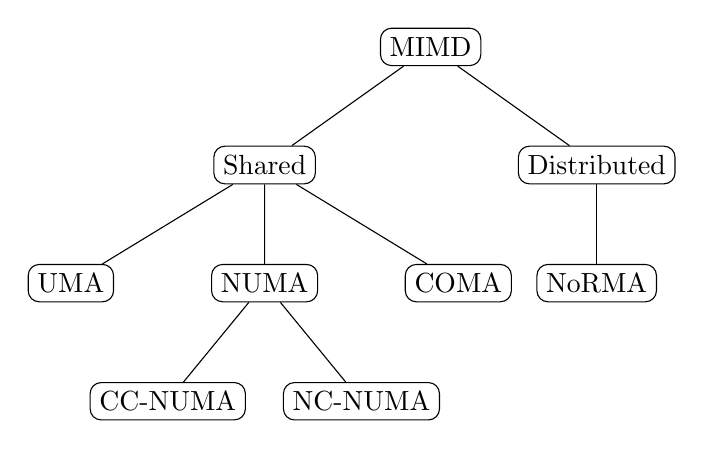
\begin{tikzpicture}[
   every node/.style = {
   level distance=1em,
   shape=rectangle, 
   rounded corners,
   draw, 
   align=center,
    top color=white%, 
   % bottom color=blue!20
   }]]
   \node {MIMD} [sibling distance=12em]
   child { node {Shared} [sibling distance=7em]
   child{node {UMA}} 
   child{node {NUMA}
   child{node {CC-NUMA}}
   child{node {NC-NUMA}}
   }
   child{node {COMA}}
   }
   child { node {Distributed}
   child { node {NoRMA}}
   };
\end{tikzpicture}
\caption{MIMD memory models}
\label{fig:1_HPC:mimd_memory_model}
\end{figure}

Those different types of memory for SIMD/MIMD model are summarized in figure~\ref{fig:1_HPC:mimd_memory_model}, and presented below.

\subsection{Shared memory} 
Several kinds of memory models are possible when it comes to multi-threaded and multi-cores execution models like MIMD or SIMD models.
We give a description of the most common shared memories architectures.
Those shared memory models are the keystone for the next parts of this study. 
Not only are they found in multi-core but also in many-core architectures with the performances are completely dependent on their usage. 

\hspace*{-2cm}
\begin{figure}
\centering 
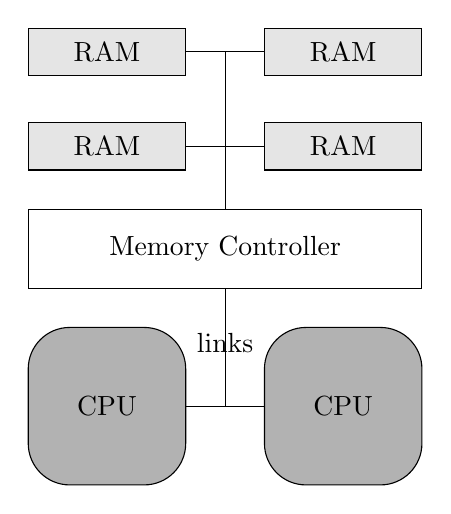
\begin{tikzpicture}
   \draw [rounded corners=15pt,fill=black!30] (0,0) rectangle (2,2) node[pos=.5] {CPU};
   \draw [rounded corners=15pt,fill=black!30] (3,0) rectangle (5,2) node[pos=.5] {CPU};

   \draw (0,2.5) rectangle (5,3.5) node[pos=.5] {Memory Controller};

   \draw (0,4) [fill=black!10] rectangle (2,4.6) node[pos=.5] {RAM};
   \draw (0,5.2) [fill=black!10] rectangle (2,5.8) node[pos=.5] {RAM};

   \draw (3,4) [fill=black!10] rectangle (5,4.6) node[pos=.5] {RAM};
   \draw (3,5.2) [fill=black!10] rectangle (5,5.8) node[pos=.5] {RAM};

   \draw [-] (2,1) -- (3,1);
   \draw [-] (2.5,1) -- (2.5,2.5);
	%\node at (2.5,2.2) {SDR, DDR, QDR};
	\node at (2.5,1.8) {links};

	\draw [-] (2.5,3.5) -- (2.5,5.5);
	\draw [-] (2,4.3) -- (3,4.3);
	\draw [-] (2,5.5) -- (3,5.5);
\end{tikzpicture}
\hspace{2cm}
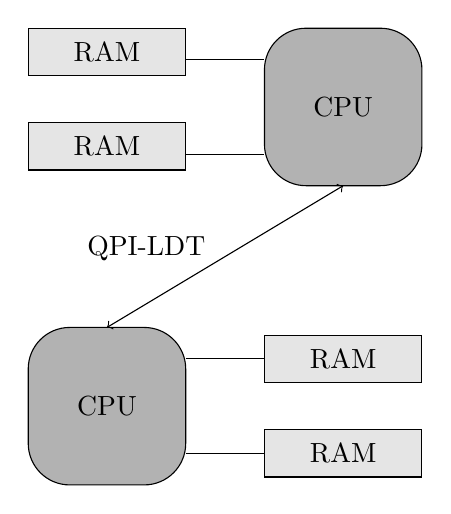
\begin{tikzpicture}
	\draw [rounded corners=15pt,fill=black!30] (0,0) rectangle (2,2) node[pos=.5] {CPU};
	\draw (3,0.1) [fill=black!10] rectangle (5,0.7) node[pos=.5] {RAM};
	\draw (3,1.3) [fill=black!10] rectangle (5,1.9) node[pos=.5] {RAM};
	\draw [-] (2,0.4) -- (3,0.4);
	\draw [-] (2,1.6) -- (3,1.6);

	\draw [rounded corners=15pt,fill=black!30] (3,3.8) rectangle (5,5.8) node[pos=.5] {CPU};
	\draw (0,4) [fill=black!10] rectangle (2,4.6) node[pos=.5] {RAM};
	\draw (0,5.2) [fill=black!10] rectangle (2,5.8) node[pos=.5] {RAM};
	\draw [-] (2,4.2) -- (3,4.2);
	\draw [-] (2,5.4) -- (3,5.4);

	\draw [<->] (1,2) -- (4,3.8);
	\node at (1.5,3) {QPI-LDT};
\end{tikzpicture}
%\hspace{1cm}
%\begin{tikzpicture}
%	\draw [rounded corners=15pt] (1,0) rectangle (3,2) node[pos=.5] {CPU};
%	\draw [rounded corners=15pt] (1,3.8) rectangle (3,5.8) node[pos=.5] {CPU};
%
%	\draw (0,2.1) rectangle (2,2.8) node[pos=.5] {RAM};
%	\draw (0,3.2) rectangle (2,3.8) node[pos=.5] {RAM};
%	
%	\draw (3,2.2) rectangle (5,2.8) node[pos=.5] {RAM};
%	\draw (3,2.2) rectangle (5,3.8) node[pos=.5] {RAM};
%
%\end{tikzpicture}
\caption{UMA vs NUMA memory models}
\label{fig:1_HPC:UMA_NUMA}
\end{figure}

\subsubsection{UMA}
\index{Unified Memory Access}
The Uniform Memory Access architecture have a global memory shared by every threads or cores. 
Every processor in UMA uses its own cache as local private memory and the accesses consume the same amount of time.
The addresses can be accessed directly by each processor which makes the access time ideal. 
The downside is that more processors require more buses and thus UMA is hardly scalable. 
Cache consistency problem also appears in this context and will be discussed in next part.
Indeed, if a data is loaded in one processor cache and modified, this information has to be spread to the memory and possibly other processes cache. 

With the rise of accelerators like GPUs and their own memory, some constructors found ways to create UMA with heterogeneous memory.
AMD created the heterogeneous UMA, hUMA~\cite{rogers2013amd} in 2013, allowed CPU and GPU to target the same memory area, but the performances still needed to be checked in an HPC context.

\subsubsection{NUMA}
\index{Non Uniform Memory Access}
In Non Uniform Memory Access every processor has access to its own private memory but allows other processors to access it though Lightning Data Transport (LDT) or Quick Path Interconnect (QPI) for Intel architectures. 

As mentioned for the UMA memory, even if the processors do not directly access to the memory cache, coherency is important. 
There are two methods possible to aid in coherency.
First, the most used is Cache-Coherent NUMA (CC-NUMA) where protocols are used to keep data coherency through the memory. 
Second, No Cache NUMA (NC-NUMA) forces the processes to avoid cache utilization and write results to main memory, losing all the benefits of caching data. 

\subsubsection{COMA}
\index{Cache-Only Memory Access}
In Cache-Only Memory Accesses, the whole memory is seen as a cache shared by all the processes processes.
A \textit{Attraction memory} pattern is used to \textit{attract} the data near the process that will use them. 
This model is less commonly used and, in best cases, leads to same results as NUMA.

\subsection{Distributed memory}
\index{No Remote Memory Access}
The previous models are dedicated to shared memory, as in the processes can access memory of their neighboring processes. 
In some cases, like supercomputers, it would be too heavy for processors to handle the requests of all the others through the network. 
Each process or node will then possesses its own local memory that can be shared only between local processes. 
In order to access to other nodes memory, communications through the network has to be done and copied into local memory. 
This distributed memory model is called No Remote Memory Access (NoRMA).
This requires transfer schemes that have to be added to local read-write accesses.

\section{Performances characterization in HPC}
Previously we described the different execution models and memory models for HPC. 
We need to be able to emphasis the performances of a computer and a cluster based on those aspects.

There can be several types of performances.
First, it can be defined by the speed of the processors themselves with the frequency defined in GHz. 
We define the notion of \textit{cycle} to be the number that determines the speed of a processor. 
This is the amount of time between two pulses of the oscillator at the best frequency with higher cycles per seconds being better. 
This can be used to estimate the highest computational power of a machine. 
The information is not perfect, however, because the ALU is not constantly busy due to memory accesses, communications or side effects. 
Therefore, we need to utilize more accurate ways to characterize performance.

\subsection{FLOPS}

\index{Floating-point Operations Per Second}

The FLoating point Operations Per Second (FLOPS) value considers the number of floating-point operations that the system will execute in a second. 
Higher FLOPS is better and is the most common scale used to consider supercomputers' computational power. 
For a cluster we can compute the theoretical FLOPS (peak) based on the processor frequency in GHz with:
\begin{equation}
FLOPS_{cluster} = \#nodes \times \frac{\#sockets}{\#node} \times \frac{\#cores}{\#socket} \times \frac{\#GHz}{\#core} \times \frac{FLOPS}{cycle}
\end{equation}
With $\#nodes$ the number of computational node of the system, $\frac{\#sockets}{\#node}$ the number of sockets (=processors) per node, $\frac{\#cores}{\#socket}$ the number of cores in the processor, $\frac{\#GHz}{\#core}$ the frequency of each core and finally $\frac{\#FLOP}{\#cycle}$ the number of floating-point operations per cycles for this architecture. 


Table~\ref{tab:1_HPC:flops_year} presents the scale of FLOPS and the year that the first world machine reached this step.
The next milestone, the exascale, is expected to be reach near 2020.  

\begin{table}
\[\arraycolsep=1.4pt\def\arraystretch{2.2}
\begin{tabular}{| l | l | l || l | l | l |}
\hline
	%\rowstyle{\bfseries}
	\textbf{Name} & \textbf{FLOPS} & \textbf{Year} & \textbf{Name} & \textbf{FLOPS} & \textbf{Year} \\
	\hline
	\hline
	kiloFLOPS & $10^{3}$ & & petaFLOPS  & $10^{15}$ & 2005 \\ 
	\hline
	megaFLOPS & $10^{6}$ & & exaFLOPS   & $10^{18}$ & 2020 ? \\
	\hline
	gigaFLOPS & $10^{9}$ & $\approx$ 1980  & zettaFLOPS & $10^{21}$ & \\
	\hline
	teraFLOPS & $10^{12}$ & 1996 & yottaFLOPS & $10^{24}$ & \\
	\hline
	\end{tabular}
	\]
	\caption{Floating-point Operation per Second and years of reach in HPC.}
	\label{tab:1_HPC:flops_year}
\end{table}


There still exists many ways to measure computer's performance such as: Instructions Per Seconds (IPS), Instructions per Cycle (IPC) or Operations Per Seconds (OPS).
However, it is hard to consider what an operation or instruction can be.
Thus, floating point can be considered as a basis, providing a comparison for performance. 


\subsection{Power consumption}
An additional way to consider machine performance is to estimate the number of operations regarding the power consumption. 
This considers all the previous metrics like FLOPS, IPS, IPC or OPS. 
Benchmarks like the Green500 consider the FLOPS delivered over the watts consumed. 
For current architectures the many-cores accelerated architectures with GPUs seems to deliver the best FLOPS per watt ratio.

This subject is the underlying goal of our study. 
Without the power consumption limit we would already be able to build exascale or even more powerful machine by combining billions and billions of nodes. 
This is not doable due to processors power consumption and cooling cost.
The question have been studied in our laboratory with the development of tools like \textit{Powmon} (Power Monitor).
This power monitor allows to instantaneously query the power consumption with CPU and GPU on a running node of a cluster. 

\subsection{Scalability}

After considering architectures evaluation, one have to measure the applications performances.
The scalability expresses the way a program reacts to parallelism. 
When an algorithm is implemented on a serial machine and is ideal to solve a problem, one may consider to use it on more than one core, socket, node or even cluster. 
Indeed, while using more resources one may expect less computation time or access larger instances, or a combination of both. 
This is completely dependent of the algorithm's parallelization and is expressed through scalability. 
A scalable program will scale on as many processors as provided, whereas a poorly scalable one will give the same, or even worst results, than the serial code.  
Scalability can be approached using speedup and efficiency.

\subsection{Speedup and efficiency}
The latency is the time required to complete a task in a program with lower latency being better. 
\index{Latency} 

The speedup compares the latency of both sequential and parallel algorithm. 
In order to get relevant results, one may consider the given best serial program against the best parallel implementation.

Considering $n$, the number of processes, and $n=1$ the sequential case.
$T_n$ is the execution time working on $n$ processes and $T_1$ the sequential execution time. 
The speedup can be defined using the latency by the formula: 
\index{Speedup}
\begin{equation}
\text{speedup} = S_n =  \frac{T_1}{T_n}
\end{equation}

\begin{figure}
\centering 
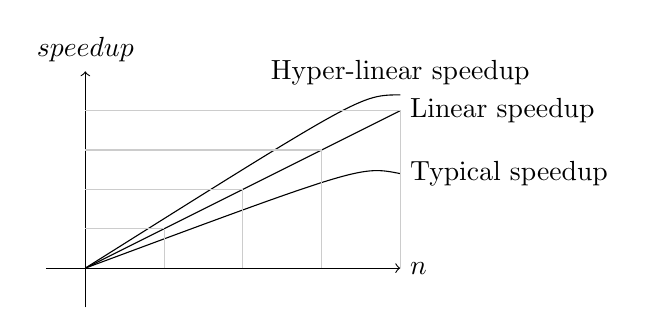
\begin{tikzpicture}
	\draw[->] (-.5,0) -- (4,0) node[right] {$n$};
	\draw[->] (0,-.5) -- (0,2.5) node[above] {$speedup$};
	\draw (0,0) -- (4,2) node[right] {\text{Linear speedup}};
	\draw (0,0) .. controls (3.5,1.3) .. (4.,1.2) node[right] {\text{Typical speedup}} ;
	\draw (0,0) .. controls (3.5,2.2) .. (4.,2.2) node[above] {\text{Hyper-linear speedup}} ;
   \draw[black!20] (1,0) -- (1,.5);
   \draw[black!20] (2,0) -- (2,1);
   \draw[black!20] (3,0) -- (3,1.5);
   \draw[black!20] (4,0) -- (4,2);
   \draw[black!20] (0,.5) -- (1,.5);
   \draw[black!20] (0,1) -- (2,1);
   \draw[black!20] (0,1.5) -- (3,1.5);
   \draw[black!20] (0,2) -- (4,2);
\end{tikzpicture}
\caption{Observed speedup: linear, typical and hyper-linear speedups}
\label{fig:1_HPC:speedup_obs}
\end{figure}


In addition to speedup, the efficiency is defined by the speedup divided by the number of workers: 
\index{Efficiency}
\begin{equation}
\text{efficiency} = E_n = \frac{S_n}{n} = \frac{T_1}{nT_n}
\end{equation}
The efficiency, usually expressed in percent, represents the evolution of the code stability to growing number of processors. 
As the number of processes grows, a scalable application will keep an efficiency near 100\%.


As shown on figure \ref{fig:1_HPC:speedup_obs} several kinds of speedup can be observed. 
\paragraph{Linear, reference speedup: }
The linear speedup usually represents the target for every program in HPC. 
To have a constant efficiency means that the speedup grows linearly as the number of processors grows is the ideal case. 
Codes fall typical into two cases: typical and hyper-linear speedup. 
\paragraph{Typical speedup: }
This represents the most common observed speedup. 
As the number of processors grows, the program faces several of the HPC walls, such as communications wall or memory wall. 
The increasing number of computational power may be lost in parallel overhead resulting in efficiency being reduced. 
\paragraph{Hyper-linear speedup: }
In some cases, we observe an hyper-linear speedup, meaning the results in parallel are even better than the ideal case. 
This increasing efficiency can occur if the program fits exactly in memory with less data on each processor or even fit perfectly for the cache utilization. 
The parallel algorithm can also be more efficient than the sequential one.
For example, if the search space in an optimized application is divided over processing units, one can find good solutions more quickly.

\subsection{Amdahl's and Gustafson's law}
The Amdahl's and Gustafson's laws are ways to evaluate the maximal possible speedup for an application taking into account different characteristics. 

\subsubsection{Amdahl's law}
\index{Amdahl's law}
The Amdahl's law\cite{amdahl1967validity} is used to find the theoretical speedup in latency of a program.
We can separate a program into two parts, the one that can be executed in parallel with optimal speedup and the one that is intrinsically sequential.
The law states that even if we reduce the parallel part using an infinity of processes the sequential part will reach 100\% of the total computation time. 

Extracted from the Amdahl paper the law can be written as: 

\begin{equation}
S_n = \frac{1}{Seq + \frac{Par}{n}}
\end{equation}

Where $Seq$ and $Par$ respectively the sequential and parallel ratio of a program $( Seq + Par = 1 )$.
Here if we use up to $n=\inf$ processes, $S_n \leq \frac{1}{Seq}$ the sequential part of the code become the most time consuming. 

And the efficiency become:
\begin{equation}
E_n = \frac{1}{n\times Seq + Par}
\end{equation}

\begin{figure}
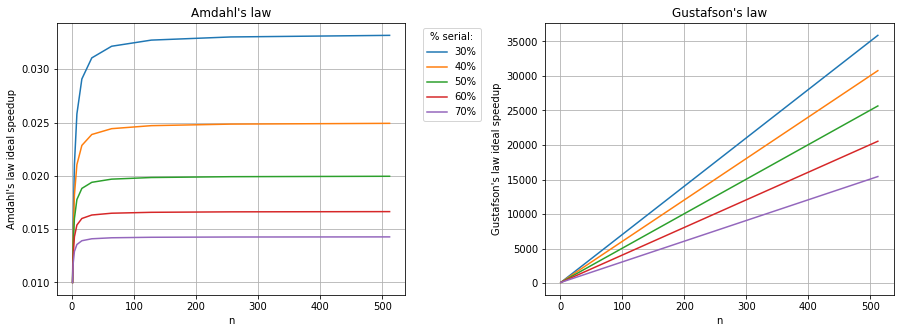
\includegraphics[width=\textwidth]{\locpath/figures/chap1/speedup_laws.png}
\caption{Theoretical speedup for Amdahl's (left) and Gustafson's (right) law}
\label{fig:1_HPC:speedup_laws}
\end{figure}

A representation of Amdahl's speedup is presented on Fig.~\ref{fig:1_HPC:speedup_laws} with varying percentage of serial part. 
%The parallel part is like $Par = (100-Ser)\%$.

\subsubsection{Gustafson's law}
\index{Gustafson's law}
The Amdahl's law focuses on time with problem of the same size. 
John L. Gustafson's idea is that using more computational units and the same amount of time, the problem size can grow accordingly. 
He considered a constant computation time with evolving problem, growing the size accordingly to the number of processes. 
Indeed the parallel part grows as the problem size does, reducing the percentage of the serial part for the overall resolution.

The speedup can now be estimated by:
\begin{equation}
S_n = Seq + Par \times n
\end{equation}

And the efficiency: 
\begin{equation}
E_n = \frac{Seq}{n} + Par
\end{equation}


Both Amdahl's and Gustafson's law are applicable and they represent two solutions to check the speedup of our applications. 
\textbf{The strong scaling}\index{Strong scaling}, looking at how the computation time vary evolving only the number of processes, not the problem size. 
\textbf{The weak scaling}\index{Weak scaling}, at the opposite to strong scaling, regards to how the computation time changes with the varying of the problem size, but keeping the same amount of work per processes. 

\section{Conclusions}

In this chapter, we presented the different basic considerations to be able to understand HPC: the Von Neumann model that is implemented in every current architecture and the Flynn taxonomy that is in constantly in evolution with new paradigms like recent SIMT from NVIDIA. 
We discussed the memory types that will be used with the different layers in our clusters, from node memory, CPU-GPGPU shared memory space to global fast shared memory. 
We finished by presenting the most important laws with Amdahl's and Gustafson's laws.
The concept of strong and weak scaling was introduced and will lead our tests through all the examples in Part II and Part III.

Those models have now to be confronted to the reality with hardware implementation and market reality, the vendors. 
The next chapter introduces chronologically hardware enhancements and their optimization, always keeping a link with the models presented in this part.

We will have to find ways to rank and characterize those architectures as there is always a gap between models and implementation. 
This will be discussed in the last chapter.

